\section{Ulteriori grafici derivanti dalle analisi con valore di $\alpha$ basso}
Nel seguente appendice, si mostrano brevemente i grafici che non sono stati inseriti direttamente nel Sezione \ref{sec:gamma}, dove sono stati discussi gli effetti che ha il parametro $\gamma$ rispetto alla distanza media che mantengono gli agenti durante l'esplorazione.

In Figura \ref{figapx:gammavsdistance}, si mostra come varia la media, calcolata su dieci simulazioni, delle distanze medie durante le simulazioni per ogni valore di $\gamma$, la media delle relative deviazioni standard e la deviazione standard massima ottenuta durante una simulazione. 
Poiché tale grafico aggrega molti dati insieme non è stato considerato significativo riportarlo nel Capitolo \ref{chap:results}.\\
\begin{figure}
	\centering
	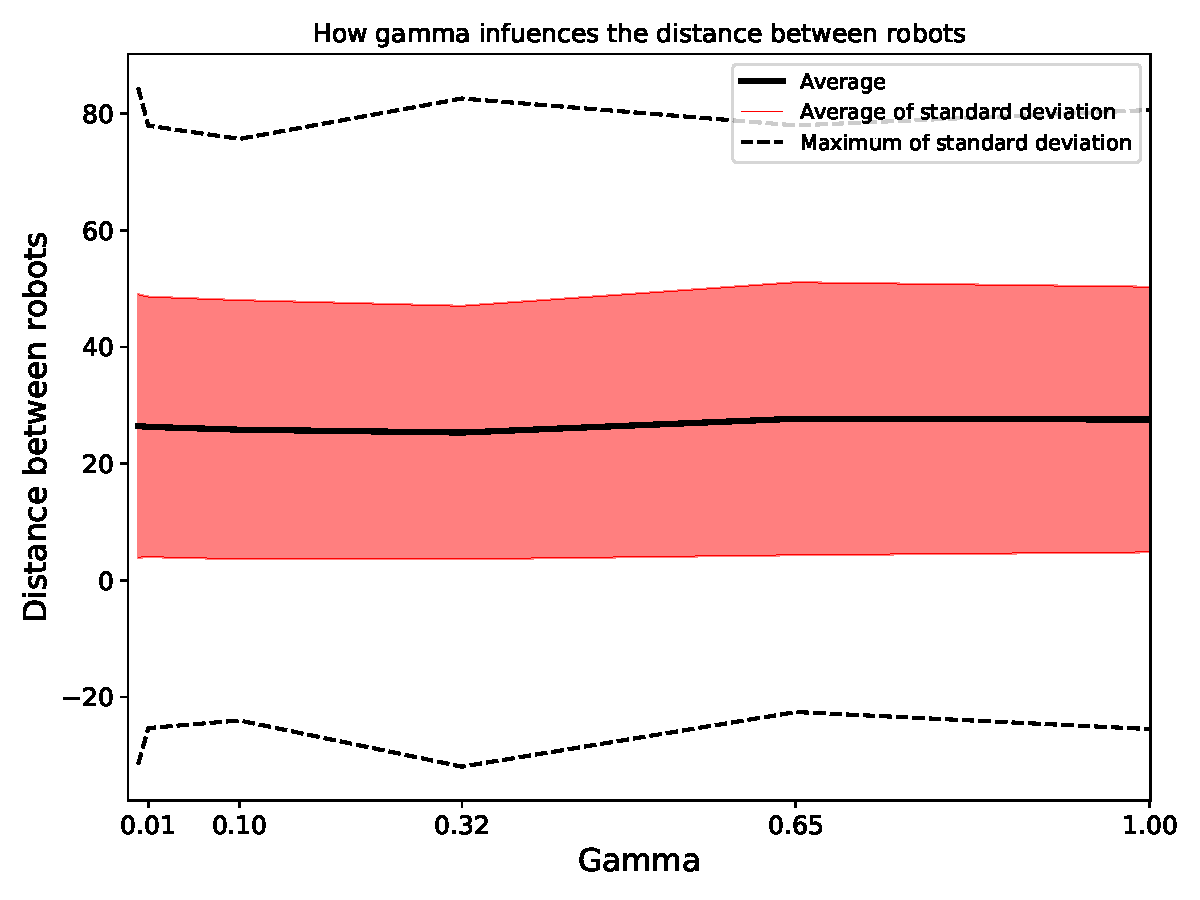
\includegraphics[width=0.9\linewidth]{images/gamma_results/low_alpha/gamma_vs_distance}
	\caption{In nero è rappresentata la media delle distanze medie mantenute durante le dieci simulazioni per ogni valore di $\gamma$, la media delle diaviozni standard calcolate per ogni simulazione e infine la riga tratteggiata rappresenta il valore massimo di deviazione standard ottenuto per ogni valore di $\gamma$.}
	\label{figapx:gammavsdistance}
\end{figure}
In Figura \ref{figapx:gammaDistr} sono mostrate le distribuzioni delle distanze medie tra gli agenti durante le simulazioni per ogni valore di $\gamma$ analizzato, in aggiunta a quelle mostrate nella Sotto-sezione \ref{subsec:gammaalow}.\\
\begin{figure}
	\begin{tabular}{cc}
		\subfloat[Distribuzione della distanza media mantenuta dai robot con un valore di $\gamma$ pari a 0.]{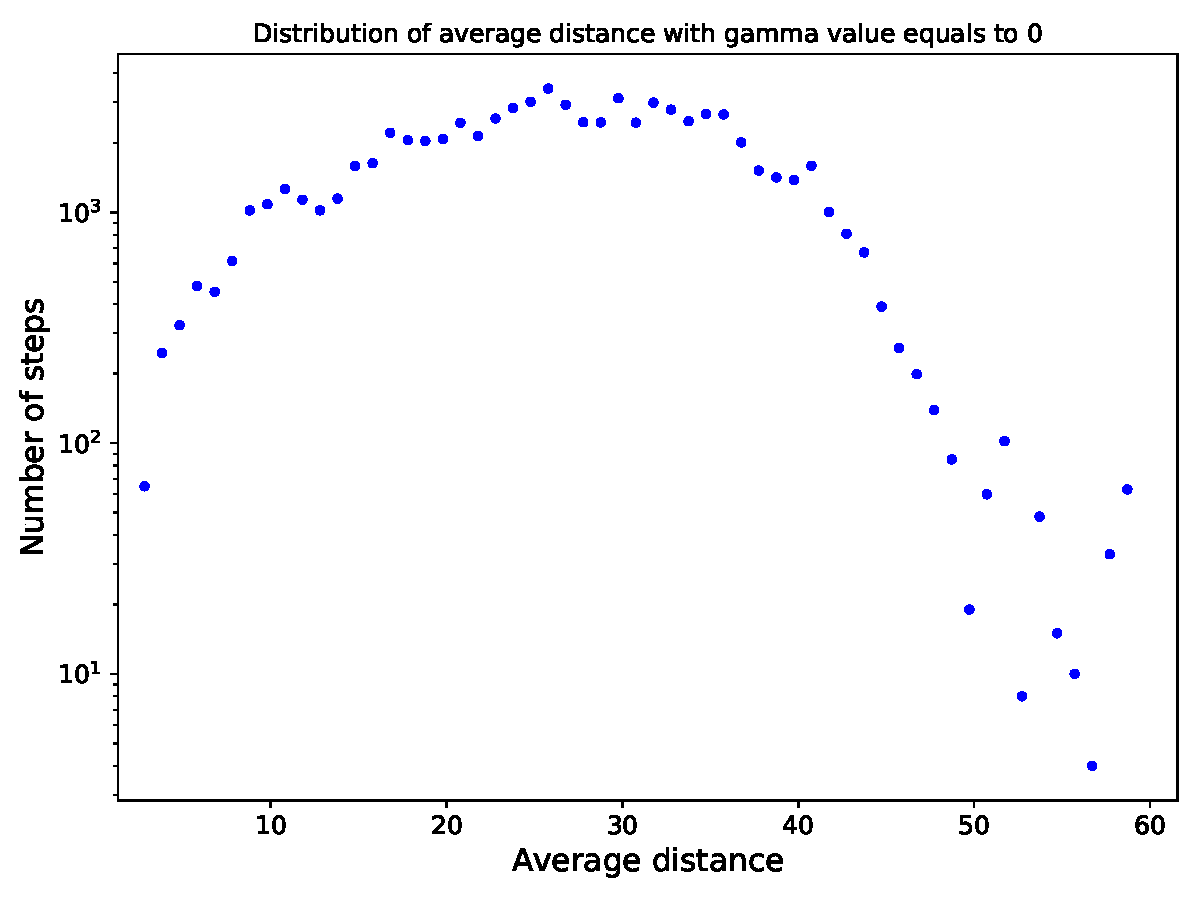
\includegraphics[width = .5\textwidth]{images/gamma_results/low_alpha/distribution_distance_gamma_0}} &
		\subfloat[Distribuzione della distanza media mantenuta dai robot con un valore di $\gamma$ pari a 0.01.]{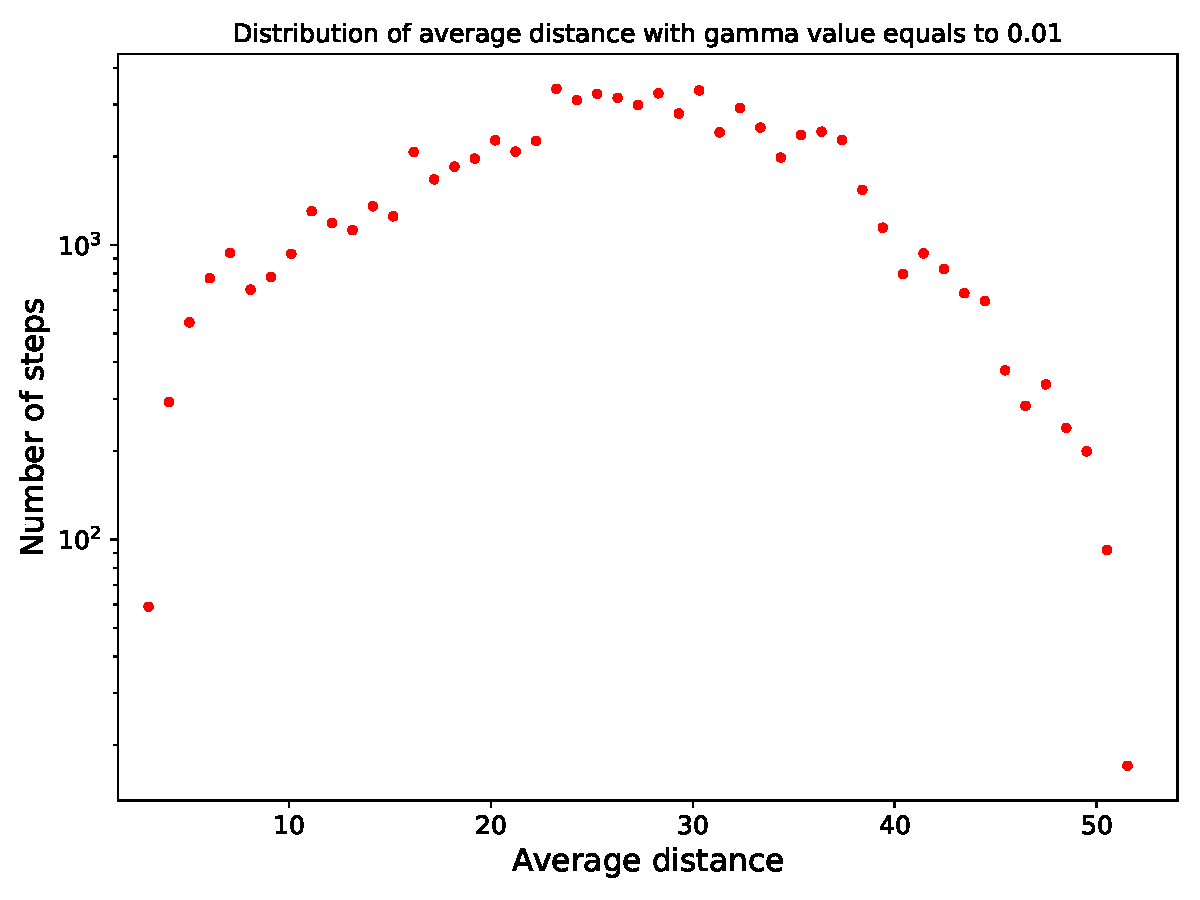
\includegraphics[width = .5\textwidth]{images/gamma_results/low_alpha/distribution_distance_gamma_0_01}}\\
		\subfloat[Distribuzione della distanza media mantenuta dai robot con un valore di $\gamma$ pari a 0.1.]{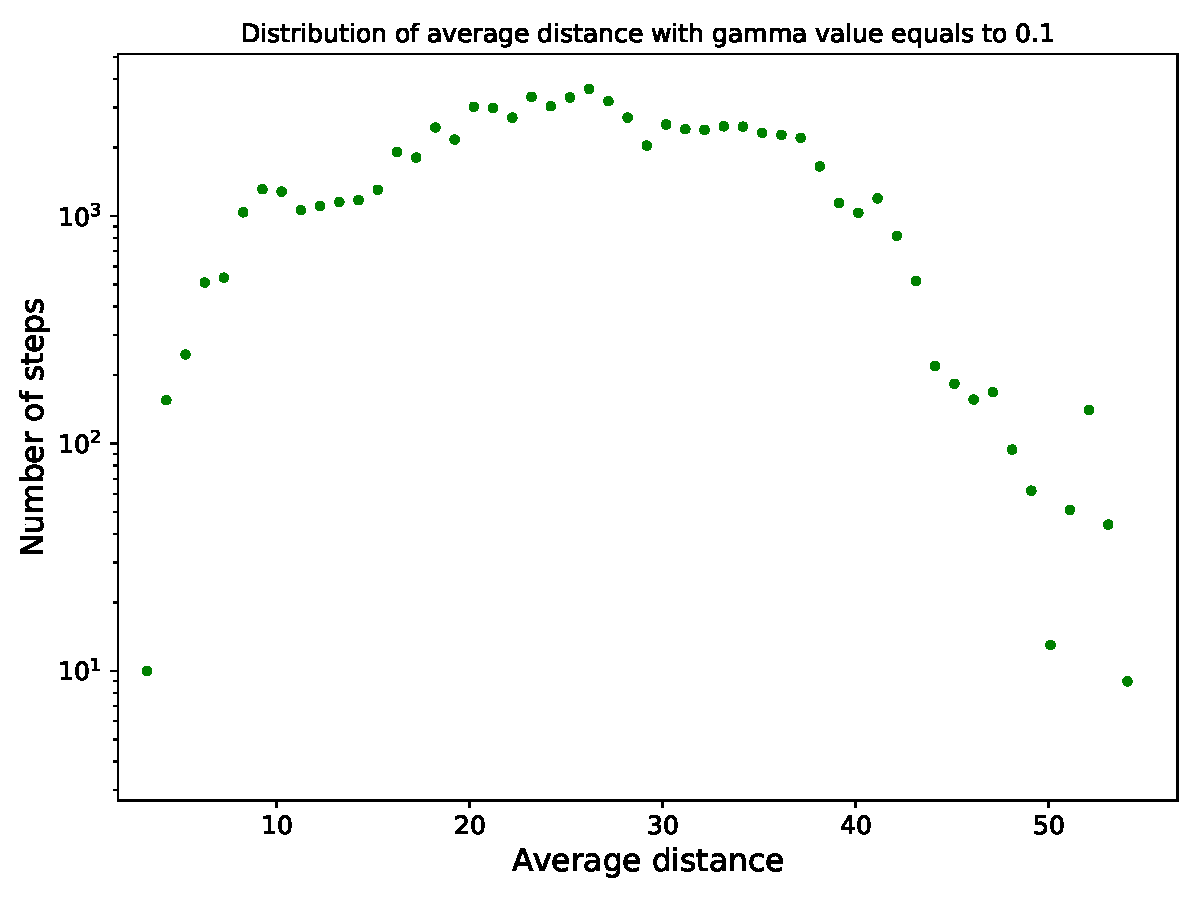
\includegraphics[width = .5\textwidth]{images/gamma_results/low_alpha/distribution_distance_gamma_0_1}} &
		\subfloat[Distribuzione della distanza media mantenuta dai robot con un valore di $\gamma$ pari a 1.]{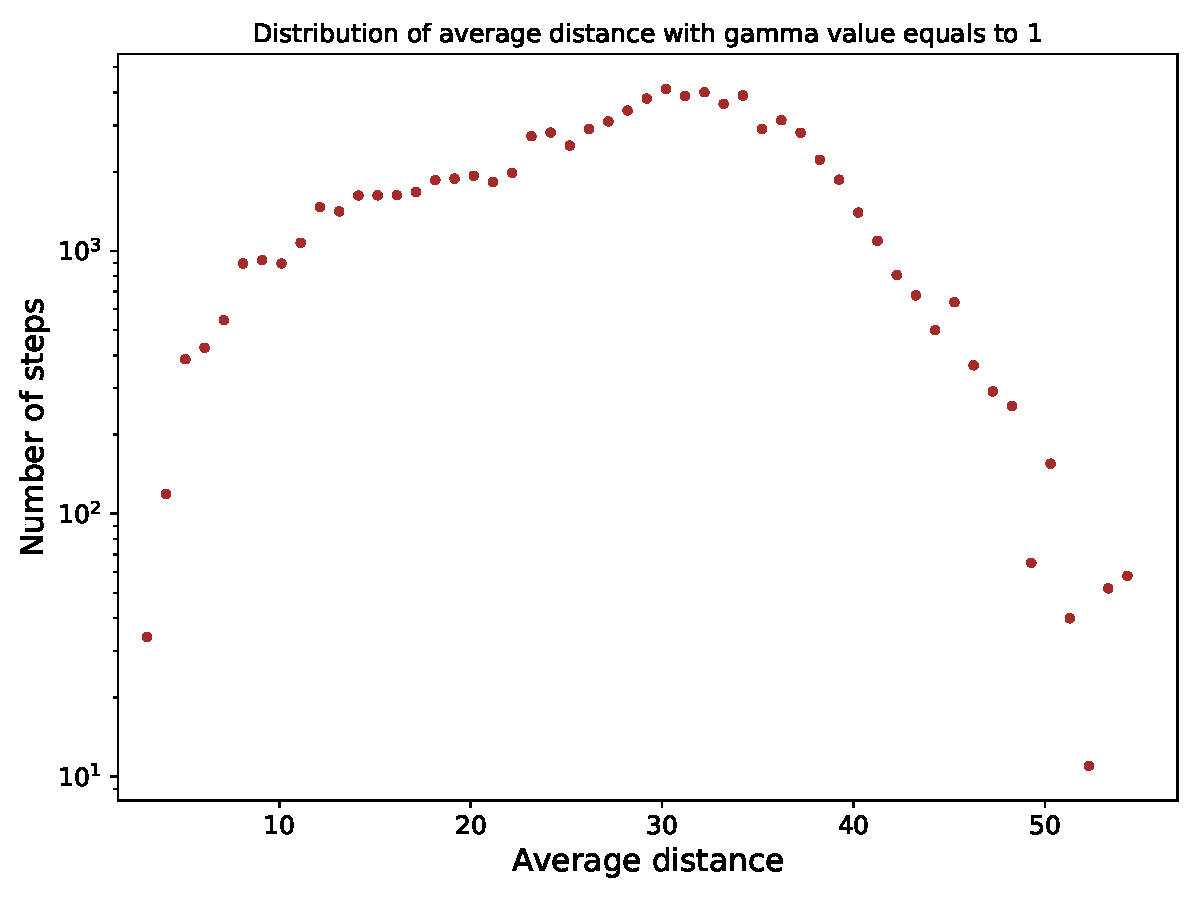
\includegraphics[width = .5\textwidth]{images/gamma_results/low_alpha/distribution_distance_gamma_1}}\\
	\end{tabular}
	\caption{Distribuzione della distanza media mantenuta dai robot al variare del valore di $\gamma$, per valutare la distribuzione si è conteggiato in quanti \textit{step} i robot hanno presentato tale distanza, il numero di \textit{bin} per produrre la distribuzione è pari alla differenza tra la distanza minima e massima presente durante la simulazione, tale valore è stato poi arrotondato. Infine si noti che l'asse delle \textit{y} è a scala logaritmica.}
	\label{figapx:gammaDistr}
\end{figure}
In Figura \ref{figapx:gammaSim} sono rappresentate le distanze medie e deviazioni standard per ogni \textit{step} di una simulazione, la simulazione è stata scelta casualmente tra le dieci effettuate per la raccolta dei dati.
\begin{figure}
	\begin{tabular}{cc}
		\subfloat[Evoluzione della distanza media tra gli agenti con un valore di $\gamma$ pari a 0.]{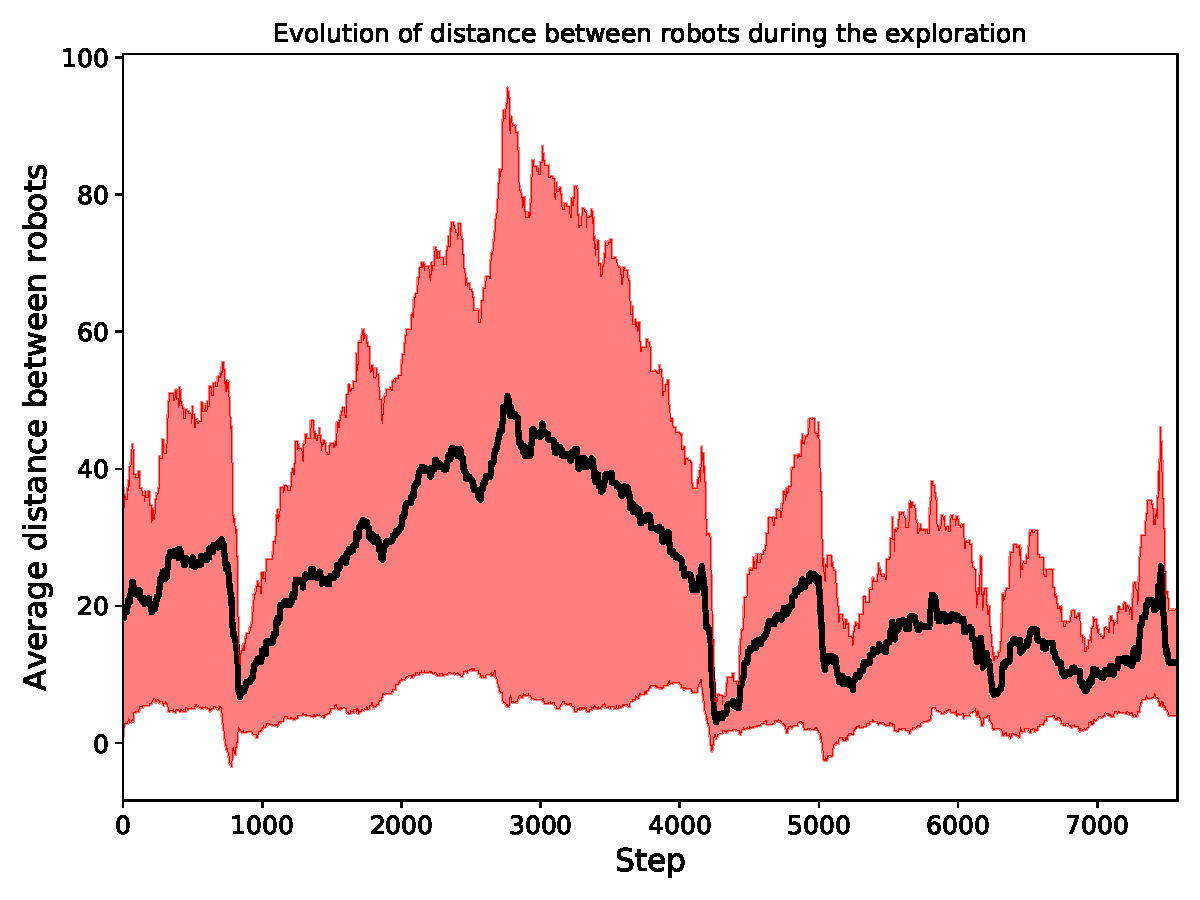
\includegraphics[width = .5\textwidth]{images/gamma_results/low_alpha/dinstance_simulation_gamma_0_simid_0}} &
		\subfloat[Evoluzione della distanza media tra gli agenti con un valore di $\gamma$ pari a 0.01.]{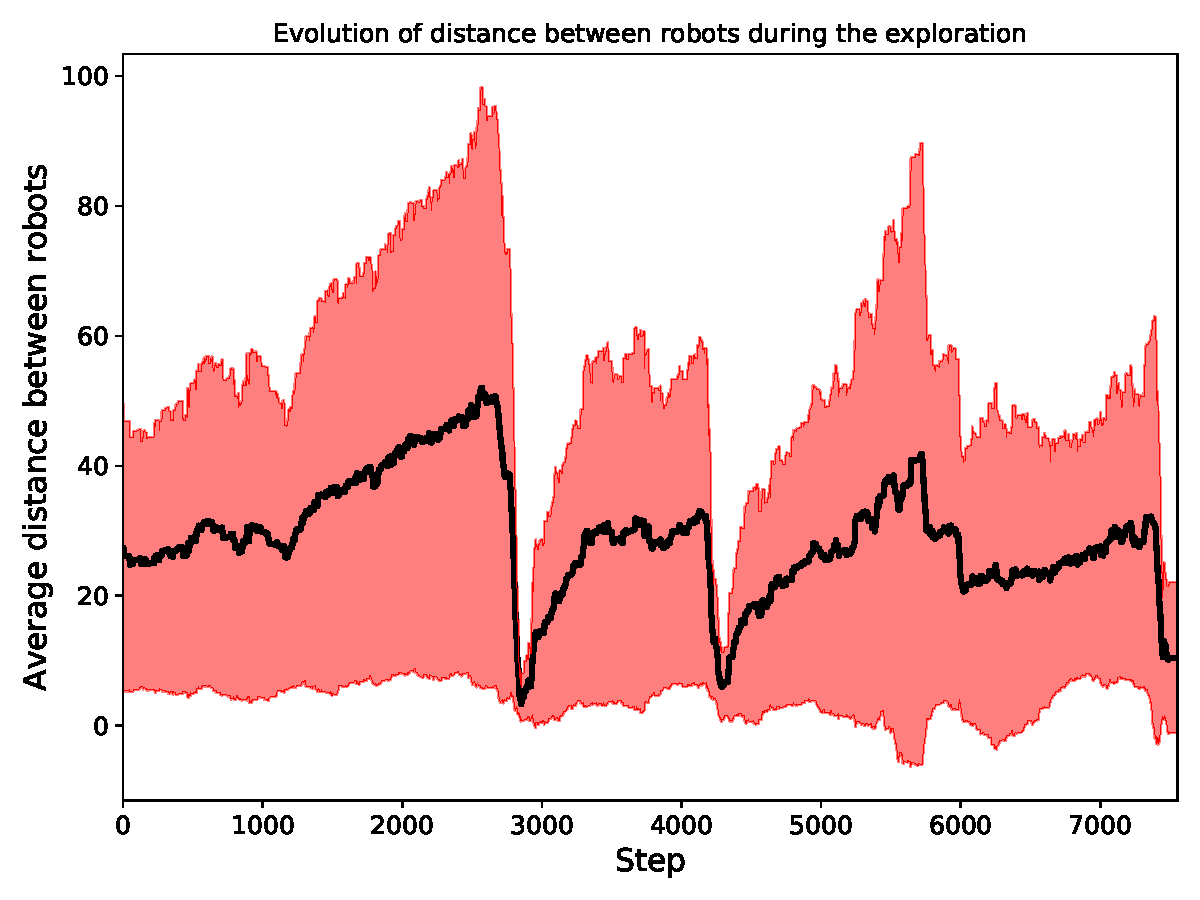
\includegraphics[width = .5\textwidth]{images/gamma_results/low_alpha/dinstance_simulation_gamma_0_01_simid_6}}\\
		\subfloat[Evoluzione della distanza media tra gli agenti con un valore di $\gamma$ pari a 0.1.]{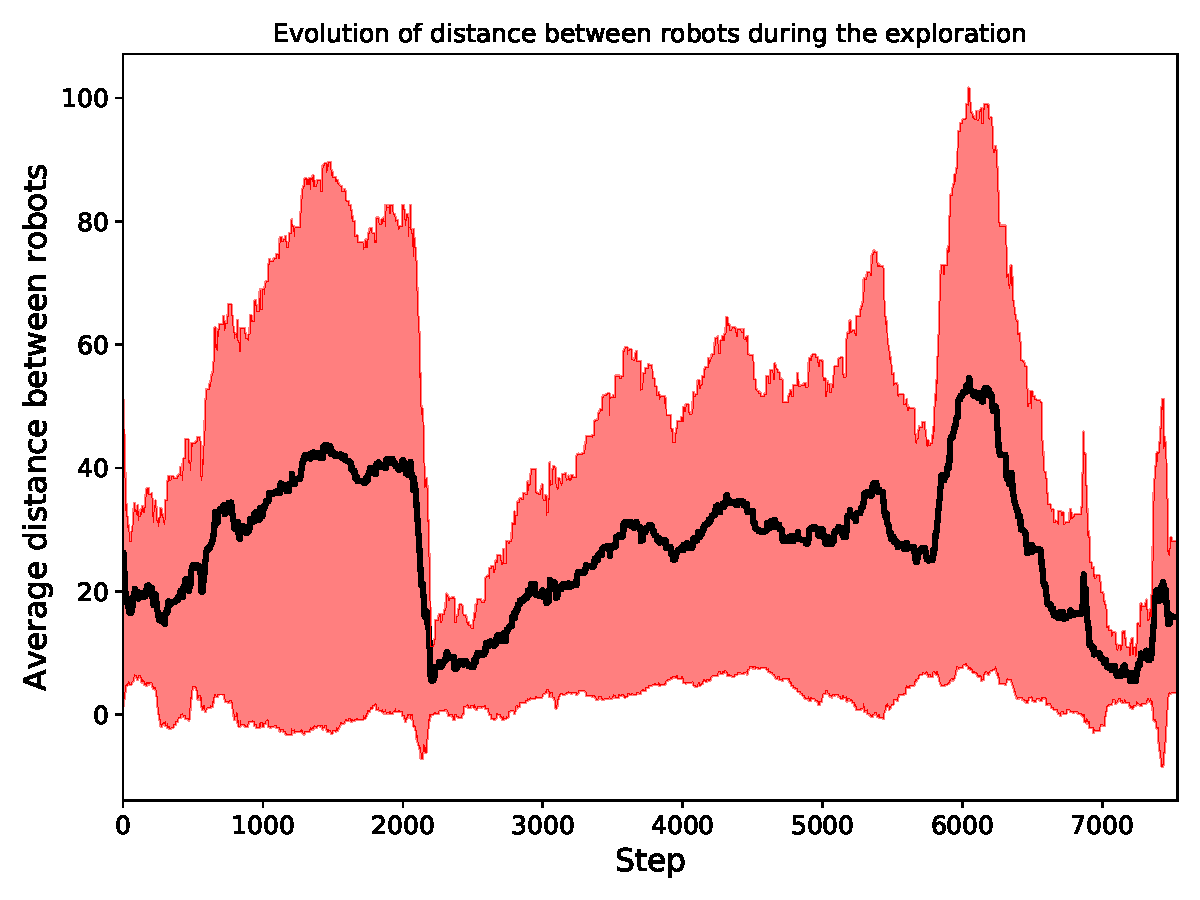
\includegraphics[width = .5\textwidth]{images/gamma_results/low_alpha/dinstance_simulation_gamma_0_1_simid_0}} &
		\subfloat[Evoluzione della distanza media tra gli agenti con un valore di $\gamma$ pari a 1.]{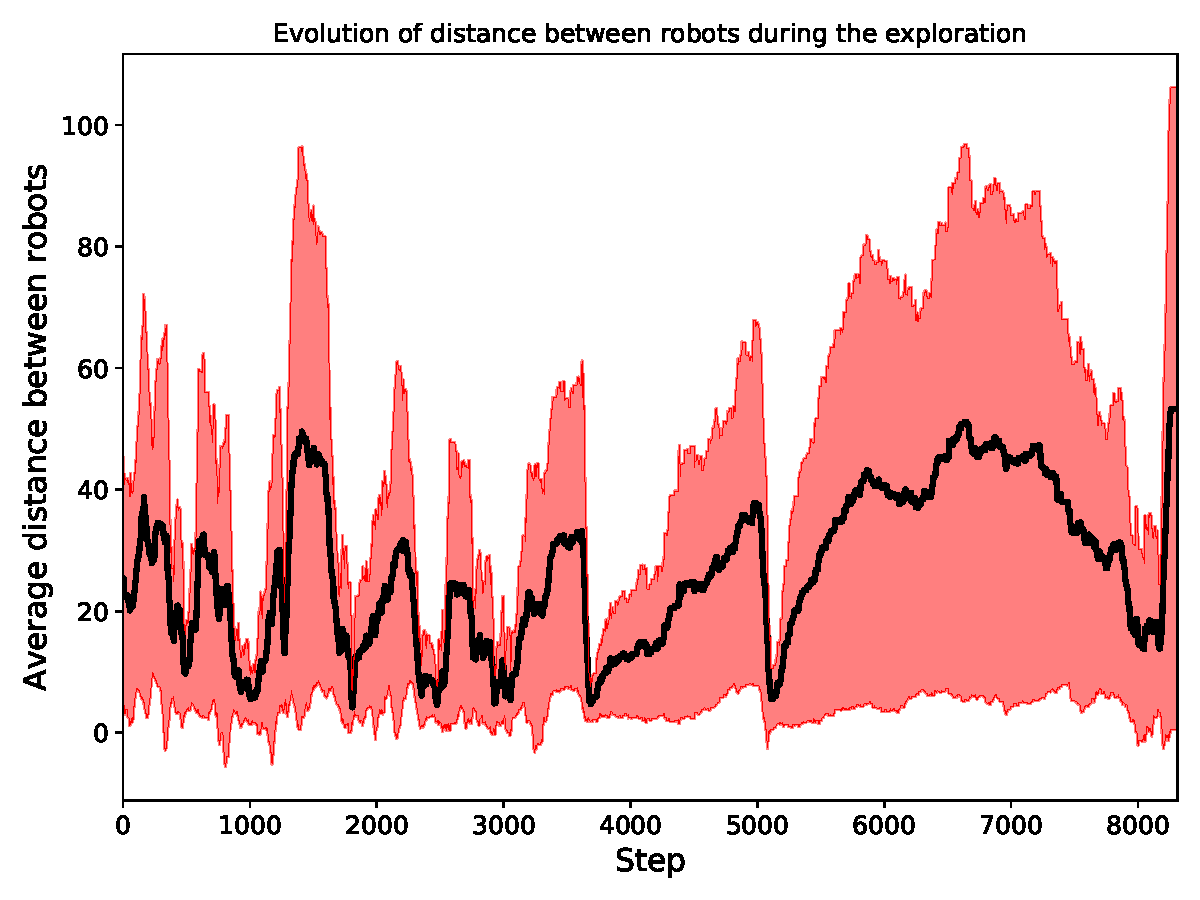
\includegraphics[width = .5\textwidth]{images/gamma_results/low_alpha/dinstance_simulation_gamma_1_simid_5}}\\
	\end{tabular}
	\caption{Sull'asse delle \textit{x} si trova il tempo, in termini di \textit{step}, impiegato per l'esplorazione della mappa, mentre sull'asse delle \textit{y} la distanza media tra gli agenti.}
	\label{figapx:gammaSim}
\end{figure}
\clearpage
\section{Ulteriori grafici derivanti dalle analisi con valore di $\alpha$ elevato}
Come in precedenza, in Figura \ref{figapx:gammavsdistanceH}, si mostra come varia la media, calcolata su dieci simulazioni, delle distanze medie durante le simulazioni per ogni valore di $\gamma$, la media delle relative deviazioni standard e la deviazione standard massima ottenuta durante una simulazione.
\begin{figure}
	\centering
	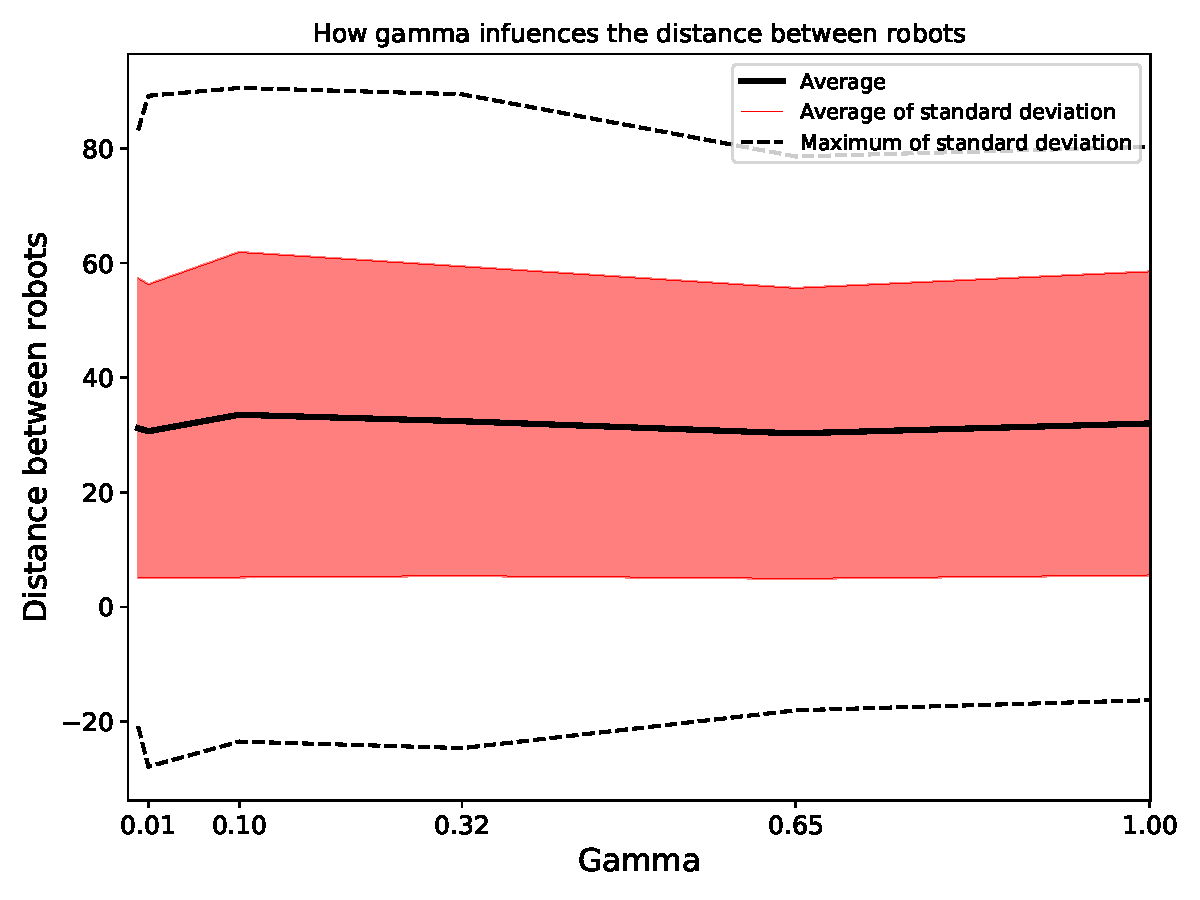
\includegraphics[width=0.9\linewidth]{images/gamma_results/high_alpha/gamma_vs_distance}
	\caption{In nero è rappresentata la media delle distanze medie mantenute durante le dieci simulazioni per ogni valore di $\gamma$, la media delle diaviozni standard calcolate per ogni simulazione e infine la riga tratteggiata rappresenta il valore massimo di deviazione standard ottenuto per ogni valore di $\gamma$.}
	\label{figapx:gammavsdistanceH}
\end{figure}
In Figura \ref{figapx:gammaHDistr} sono mostrate le distribuzioni delle distanze medie tra gli agenti durante le simulazioni per ogni valore di $\gamma$ analizzato, in aggiunta a quelle mostrate nella Sotto-sezione \ref{subsec:gammaahigh}.\\
\begin{figure}
	\begin{tabular}{cc}
		\subfloat[Distribuzione della distanza media mantenuta dai robot con un valore di $\gamma$ pari a 0.]{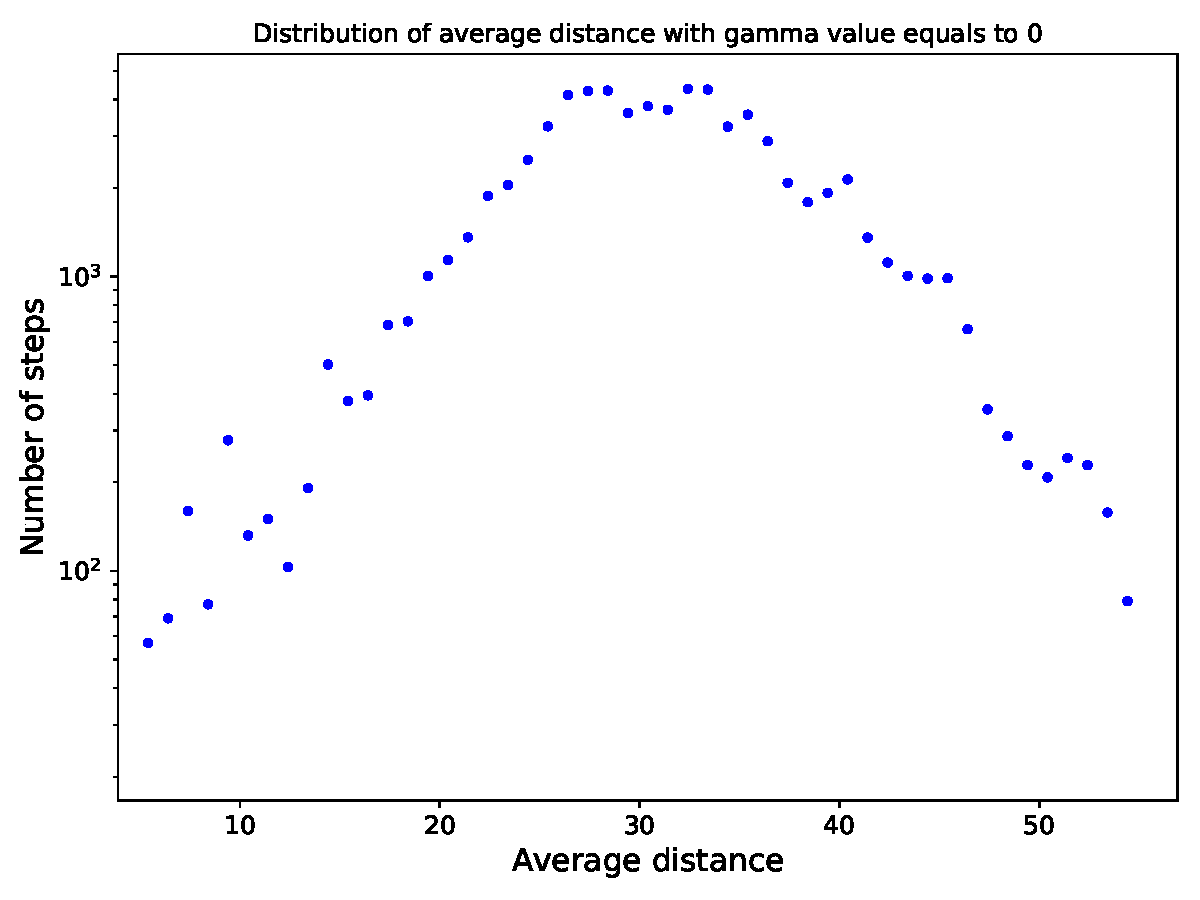
\includegraphics[width = .5\textwidth]{images/gamma_results/high_alpha/distribution_distance_gamma_0}} &
		\subfloat[Distribuzione della distanza media mantenuta dai robot con un valore di $\gamma$ pari a 0.01.]{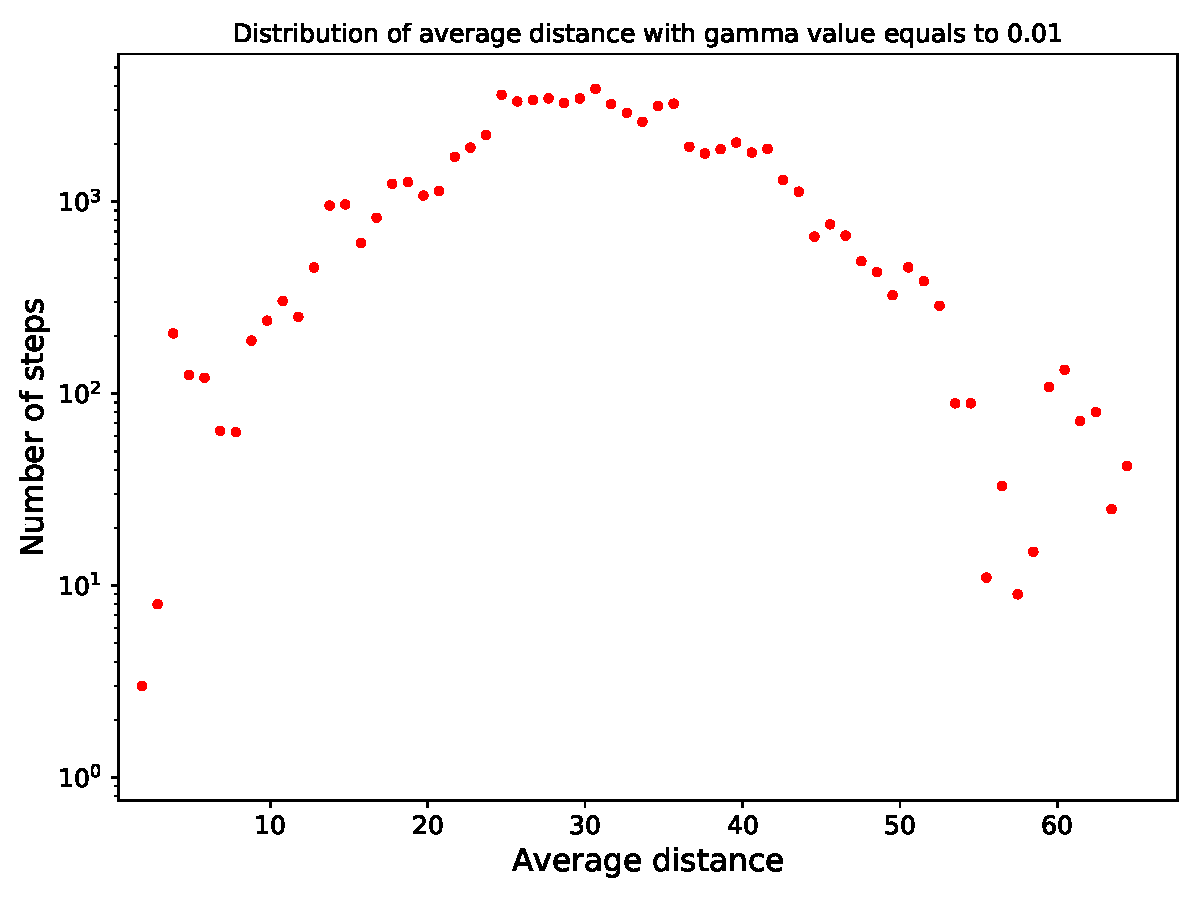
\includegraphics[width = .5\textwidth]{images/gamma_results/high_alpha/distribution_distance_gamma_0_01}}\\
		\subfloat[Distribuzione della distanza media mantenuta dai robot con un valore di $\gamma$ pari a 0.1.]{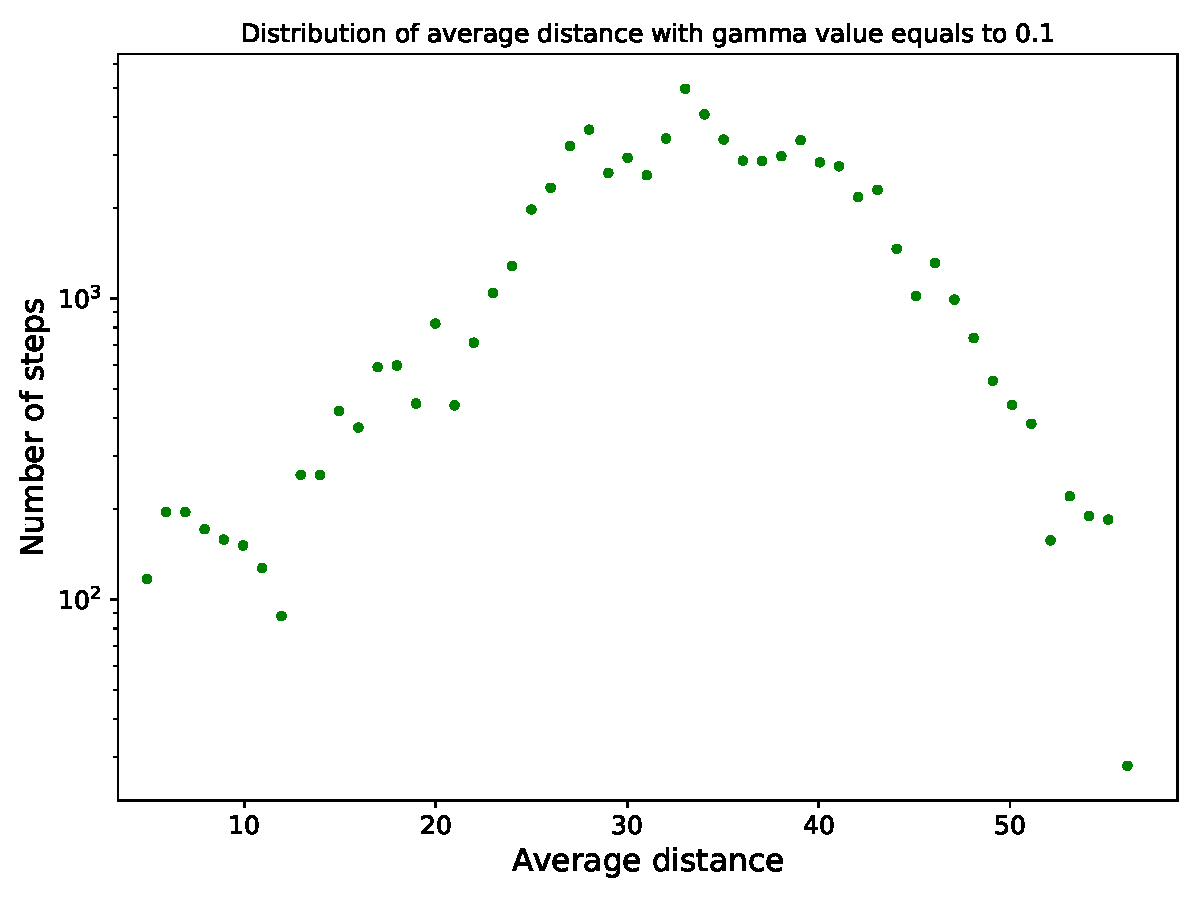
\includegraphics[width = .5\textwidth]{images/gamma_results/high_alpha/distribution_distance_gamma_0_1}} &
		\subfloat[Distribuzione della distanza media mantenuta dai robot con un valore di $\gamma$ pari a 1.]{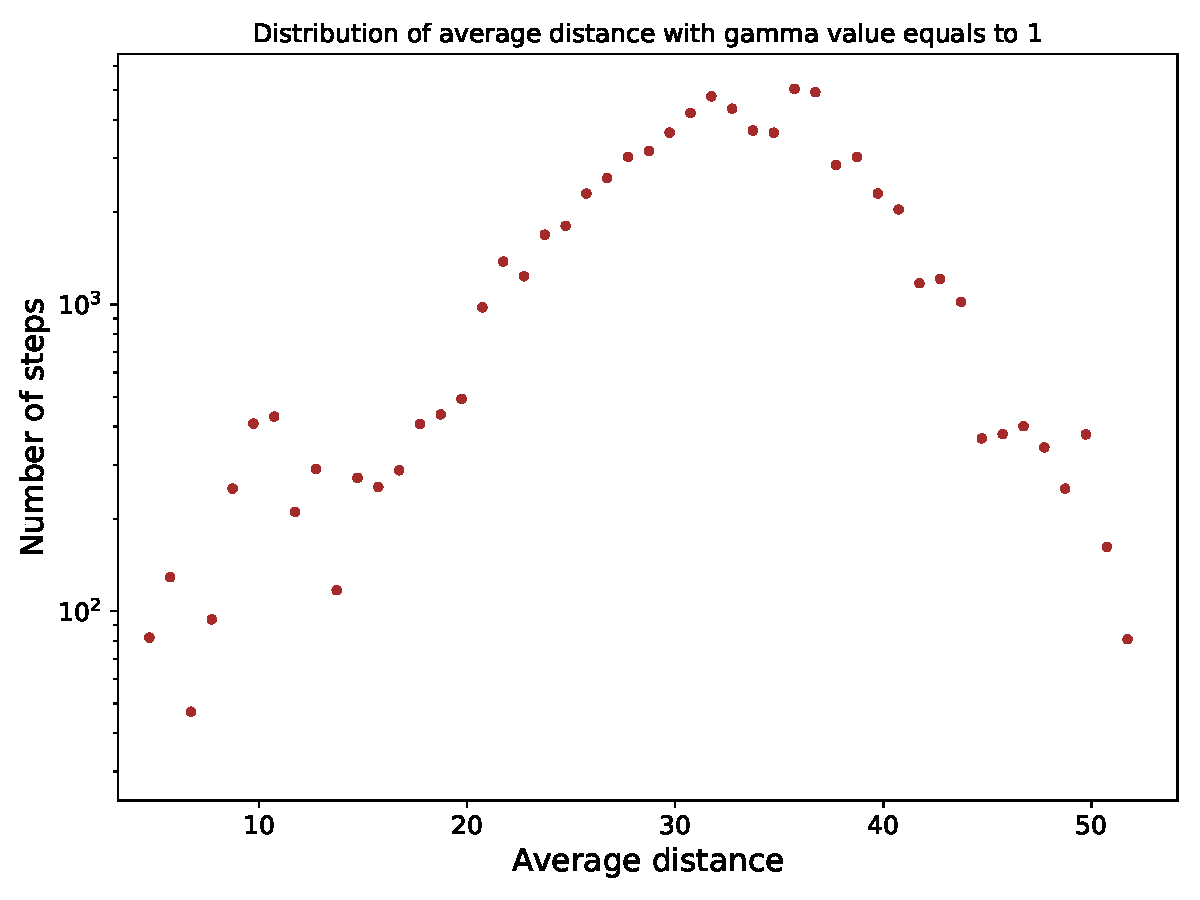
\includegraphics[width = .5\textwidth]{images/gamma_results/high_alpha/distribution_distance_gamma_1}}\\
	\end{tabular}
	\caption{Distribuzione della distanza media mantenuta dai robot al variare del valore di $\gamma$, per valutare la distribuzione si è conteggiato in quanti \textit{step} i robot hanno presentato tale distanza, il numero di \textit{bin} per produrre la distribuzione è pari alla differenza tra la distanza minima e massima presente durante la simulazione, tale valore è stato poi arrotondato. Infine si noti che l'asse delle \textit{y} è a scala logaritmica.}
	\label{figapx:gammaHDistr}
\end{figure}
In Figura \ref{figapx:gammaHSim} sono rappresentate le distanze medie e deviazioni standard per ogni \textit{step} di una simulazione, la simulazione è stata scelta casualmente tra le dieci effettuate per la raccolta dei dati.
\begin{figure}
	\begin{tabular}{cc}
		\subfloat[Evoluzione della distanza media tra gli agenti con un valore di $\gamma$ pari a 0.]{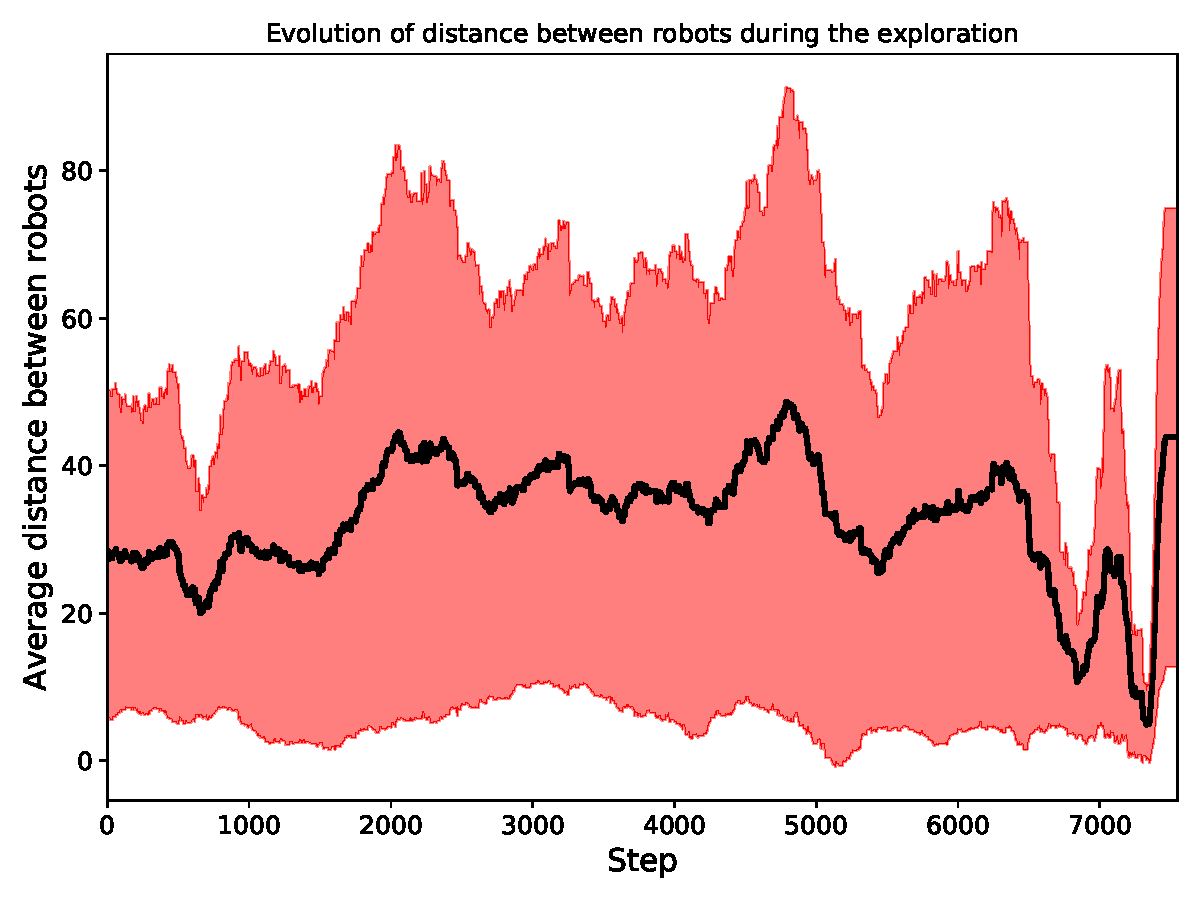
\includegraphics[width = .5\textwidth]{images/gamma_results/high_alpha/dinstance_simulation_gamma_0_simid_9}} &
		\subfloat[Evoluzione della distanza media tra gli agenti con un valore di $\gamma$ pari a 0.01.]{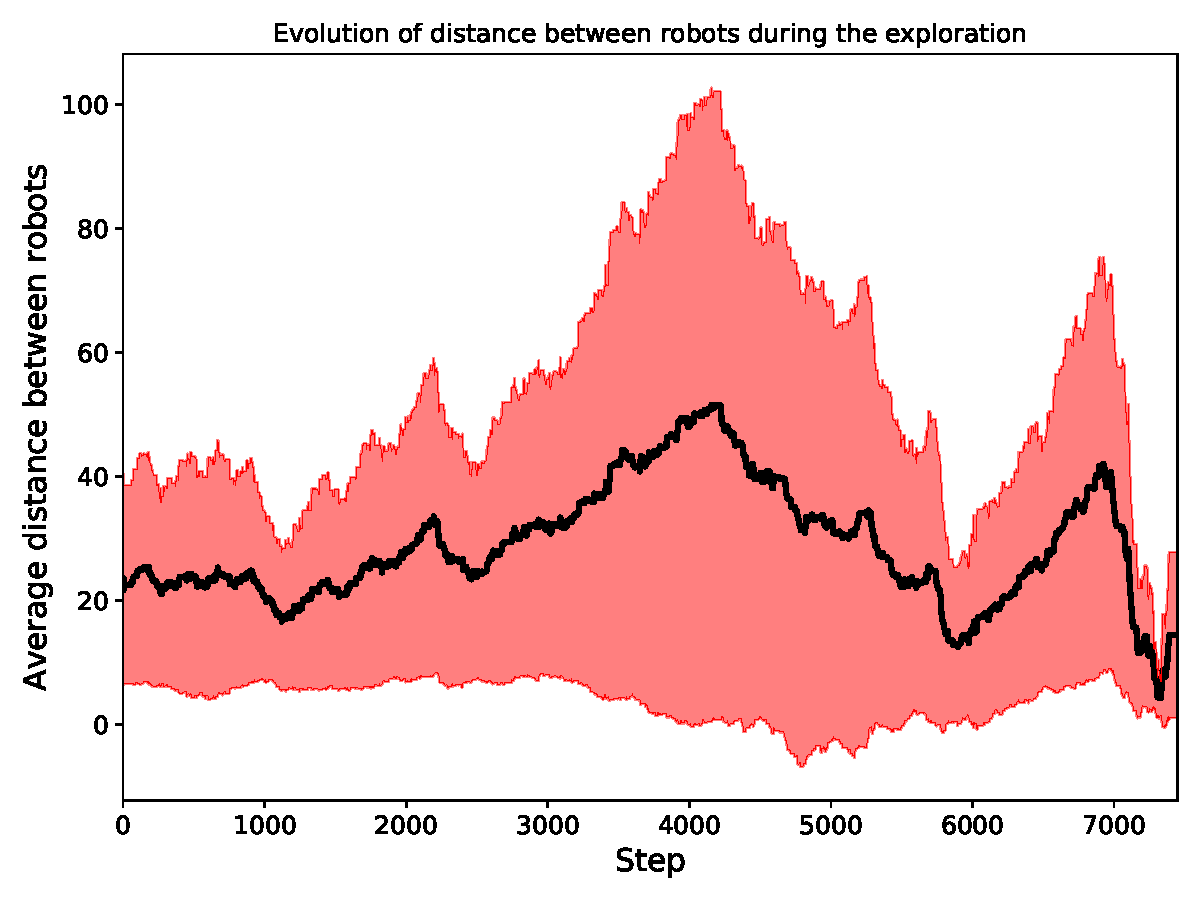
\includegraphics[width = .5\textwidth]{images/gamma_results/high_alpha/dinstance_simulation_gamma_0_01_simid_6}}\\
		\subfloat[Evoluzione della distanza media tra gli agenti con un valore di $\gamma$ pari a 0.1.]{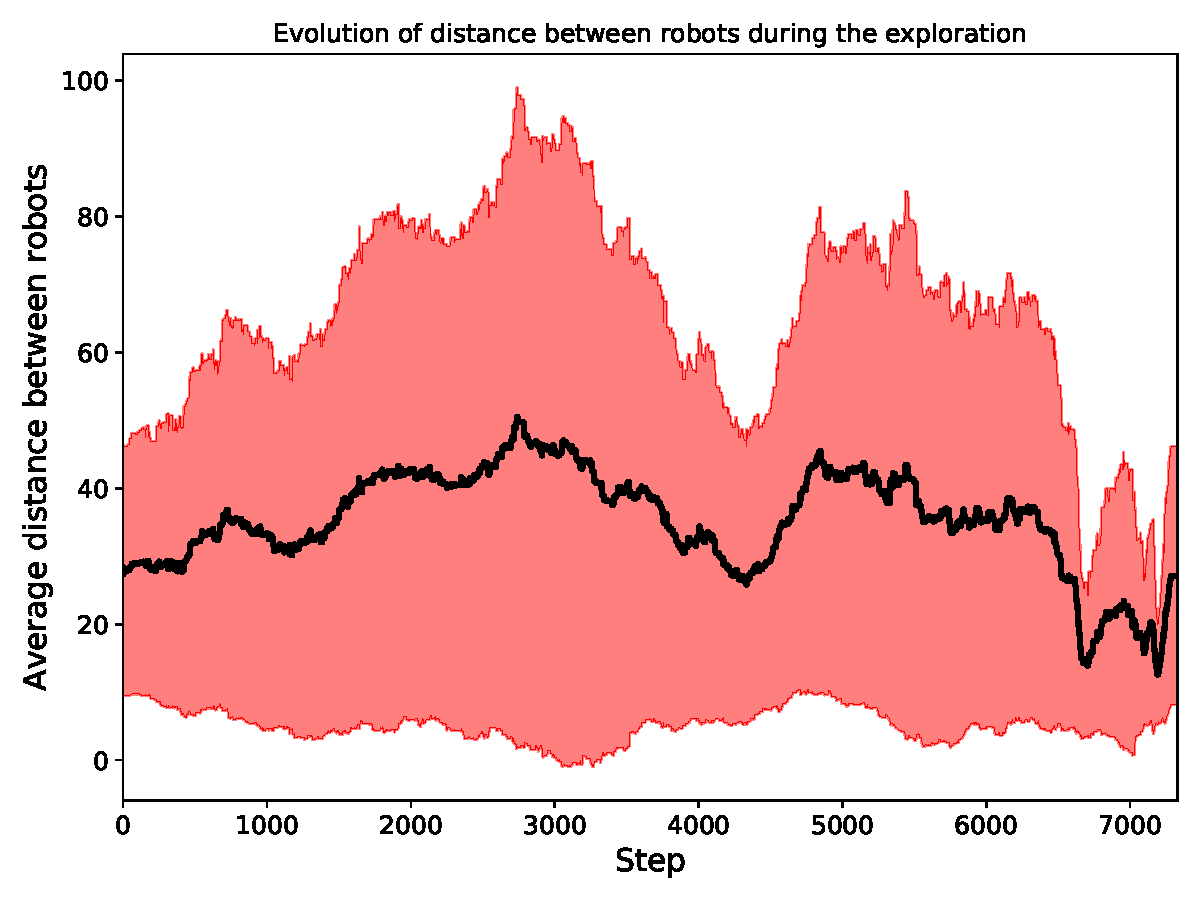
\includegraphics[width = .5\textwidth]{images/gamma_results/high_alpha/dinstance_simulation_gamma_0_1_simid_5}} &
		\subfloat[Evoluzione della distanza media tra gli agenti con un valore di $\gamma$ pari a 1.]{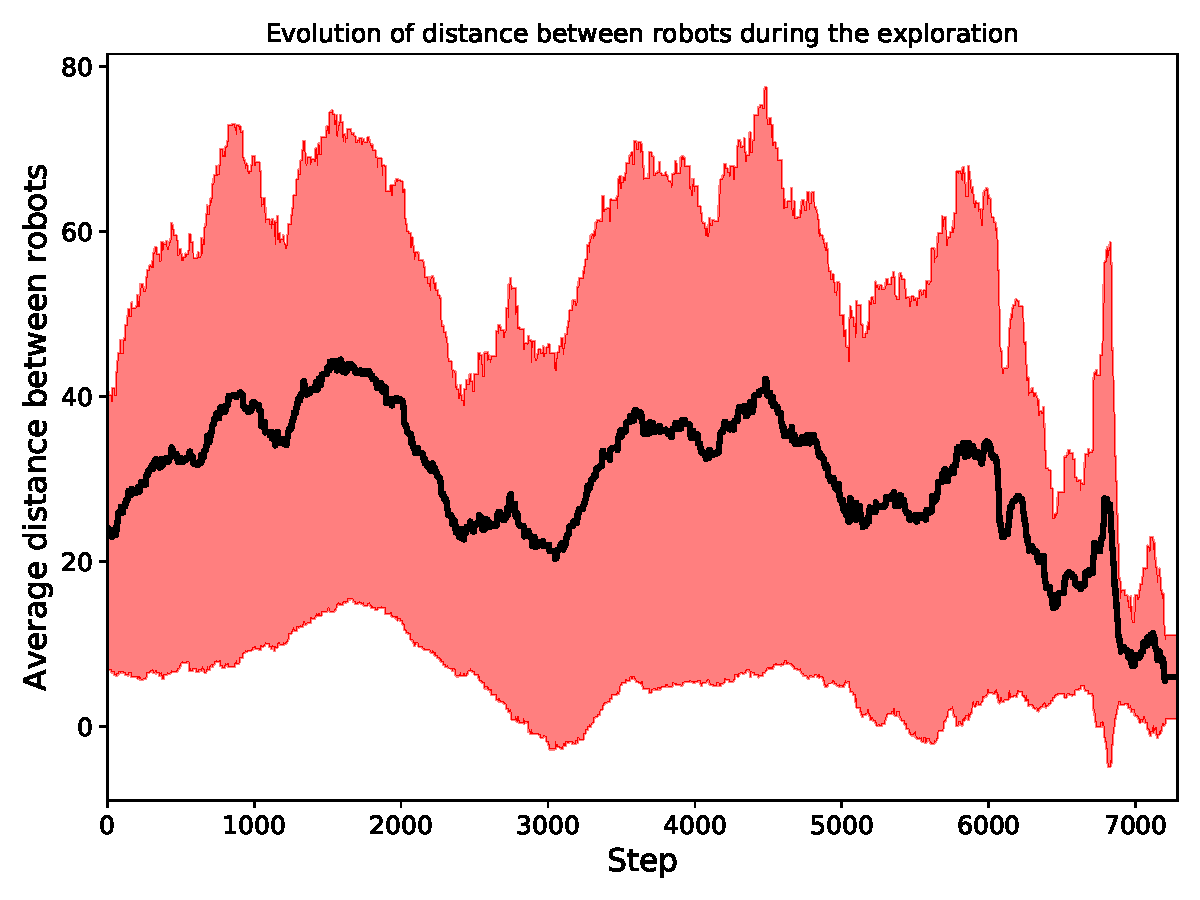
\includegraphics[width = .5\textwidth]{images/gamma_results/high_alpha/dinstance_simulation_gamma_1_simid_3}}\\
	\end{tabular}
	\caption{Sull'asse delle \textit{x} si trova il tempo, in termini di \textit{step}, impiegato per l'esplorazione della mappa, mentre sull'asse delle \textit{y} la distanza media tra gli agenti.}
	\label{figapx:gammaHSim}
\end{figure}